\documentclass[a4paper]{article}

% Pacotes para o português.
\usepackage[brazilian]{babel}
\usepackage[utf8]{inputenc}
\usepackage[T1]{fontenc}

\usepackage{sbc-template}

\usepackage{datetime}
\usepackage{graphicx}
\usepackage{float}
\usepackage{indentfirst}
\usepackage{amssymb}
\usepackage{multirow}
\usepackage[nottoc]{tocbibind}

% Espaçamento duplo. 
\usepackage{setspace}
 % Breaklines nas citações.
\usepackage{cite}

% Linha horizontal.
\newcommand{\HRule}{\rule{\linewidth}{0.5mm}}
\newcommand{\hRule}{\rule{4.5cm}{0.1mm}}

% Listagens.
\newfloat{program}{thp}{lop}
\floatname{program}{Listagem}

% Figuras.
\newcommand{\figurex}[5]
{
\begin{figure}[htb, h!]
   	\setlength{\unitlength}{1.0cm}
   	\centering
   	\includegraphics[scale=#1]{./img/#2.#3}
	\begin{center}
	   	\parbox{.9\linewidth}{\footnotesize \sf \caption{#5}  \label{#4}}
	\end{center}
\end{figure}
}

\newcommand{\ck}[0]
{
\checkmark
}

\hyphenation{}

\begin{document}

%\doublespacing
\onehalfspacing

\begin{titlepage}
\begin{center}	

% Topo 1.
\textsc{\Large UNIVERSIDADE FEDERAL DE ITAJUBÁ\\
	INSTITUTO DE MATEMÁTICA E COMPUTAÇÃO}\\[0.7cm]

% Topo 2.
\textsc{DEPARTAMENTO DE MATEMÁTICA E COMPUTAÇÃO}\\[2.8cm]

% Título.
\textsc{\Large Seminário}\\
\HRule \\[0.4cm]
{\Large \bfseries Título da Monografia}
\HRule \\[0.4cm]
\textsc{Disciplina X}\\[2.8cm]

% Etc.
\begin{minipage}{0.4\textwidth}
\begin{flushleft} \large
\emph{Alunos:}\\[0.43cm]
%\hRule\\
Aluno 1\\
Aluno 2\\
Aluno 3\\
Aluno 4\\
\end{flushleft}
\end{minipage}
\begin{minipage}{0.4\textwidth}
\begin{flushright} \large
\emph{Professor:}\\[0.4cm]
%\hRule\\
Bruno Guazzelli Batista
\end{flushright}
\end{minipage}

\vfill

\today
	
\end{center}
\end{titlepage}

\thispagestyle{empty}

\section*{Resumo}
Inserir resumo

\newpage
\pagenumbering{Roman}
\tableofcontents
\newpage
\pagenumbering{arabic}

\section{Exemplo Figura}



\begin{figure}[!htb]
\centering
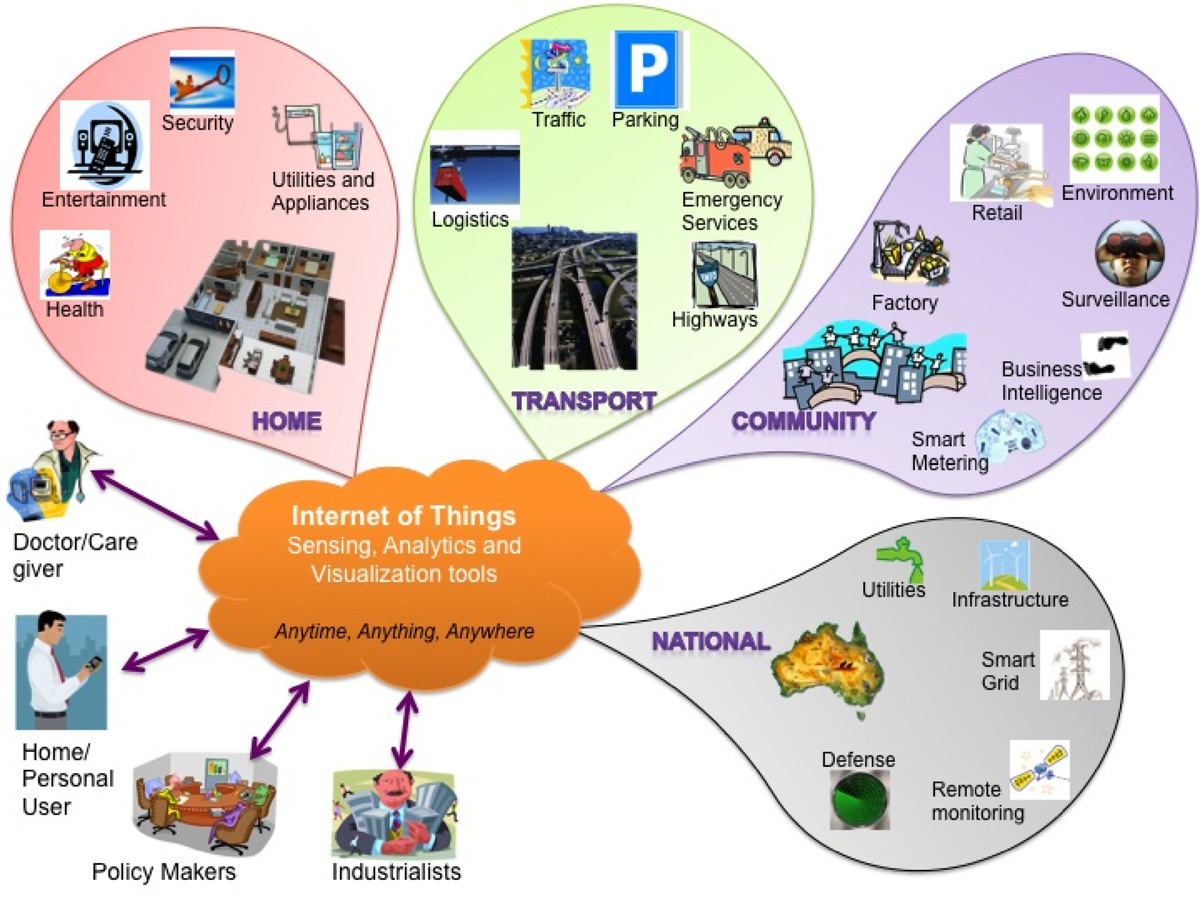
\includegraphics[width=\linewidth]{img//ilustracaoiot.png}
\caption{Internet das Coisas \cite{gubbi2013internet} \label{figure1}}
\end{figure}



\subsection{Exemplo Tabela}

As principais atividades previstas para o desenvolvimento do projeto são descritas a seguir. A Tabela~\ref{tab-crono} ilustra a organização desses itens durante o tempo de projeto.

\begin{table}[ht]
\center
\caption{Organização das atividades} \label{tab-crono}
\bf
\begin{tabular}{|c|c|c|c|c|c|c|c|c|c|c|c|c|c|c|}
\hline 
\multirow{3}{*}{Fases} & \multicolumn{6}{|c|}{Período (por bimestres)} \\ 
\cline{2-7}
 & \multicolumn{6}{|c|}{{\scriptsize 2017}} \\ 
\cline{2-7}
 & {\scriptsize 1} & {\scriptsize 2} & {\scriptsize 3} & {\scriptsize 4} & {\scriptsize 5} & {\scriptsize 6} \\ 
\hline 
1 & \ck & \ck & \ck & \ck & \ck & \ck \\ 
\hline 
2 &     &     & \ck & \ck & \ck &  \\ 
\hline 
3 &     &     & \ck & \ck & \ck &  \\ 
\hline 
4 &     &     &     & \ck & \ck & \ck\\ 
\hline 
\end{tabular}
\end{table}

\begin{enumerate}

	\item {\bf Análise crítica dos trabalhos relacionados:} estudo de mecanismos de controle de acesso disponíveis na literatura. Deve ocorrer durante todo o desenvolvimento do projeto, uma vez que novas soluções são propostas todos os dias;
	\item {\bf Implementação dos algoritmos:} implementação dos algoritmos de controle de acesso e análise da viabilidade de proposta de uma nova metodologia;
	\item {\bf Testes, coleta e análise de resultados:} realização de testes e avaliações de desempenho a fim de extrair resultados do comportamento do ambiente analisado;
	\item {\bf Elaboração de artigos científicos:} Preparação de artigos que promovam a divulgação dos resultados alcançados e a apresentação das contribuições científicas.

\end{enumerate}

%*********************************************************************************************

%\newpage
\bibliographystyle{apalike}
\bibliography{bibliography}

\end{document}